\subsubsection{Deirochelys --- Chicken Turtle}
\begin{center}
\begin{longtabu} to \textwidth {| | p{3.5cm} | X | |}

	\hline
	Taxonomy/Ancestry &
	subfamily Deirochelyinae. monotypic genus --- \emph{D. reticularia}. known as ``chicken turtles" b/c they taste like chicken.
	
	\begin{center} 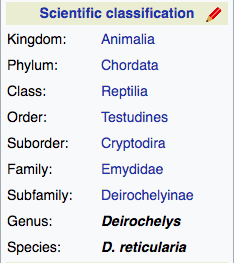
\includegraphics[scale=0.5]{testudines/emydidae/deirochelys/tax} \end{center}
	 \\
	\hline
	Size & 
	10.5-25.4 cm long
	\\
	\hline
	Color &
	yellow stripe on forelegs and rear legs. net-like pattern on carapace.
	 \\
	\hline
	Anatomy &
	it can be distinguished from the painting turtle by the unusually long, striped neck. pear-shaped carapace. it can live for 15 years.
	 \\
	\hline
	Dimorphism & 
	females are larger than males. males have a longer, thicker tail and longer front claws.
	\\
	\hline
	Behavior & 
	\begin{itemize}[noitemsep]
		\item occasionally bask
		\item spend most time in water
		\item nearly all males, some females leave wetland each fall to spend winter buried in forest, making it one of the most terrestrial turtle species
		\item aestivates* in uplands during droughts, rather than migrating 
	\end{itemize}
	\\
	\hline
	Habitat & 
	semiaquatic, it prefers quiet, still bodies of water such as shallow ponds/lakes, ditches, marshes, cypress swamps, and Carolina bays. it favors dense vegetation, and soft substrate. it is tolerant of ephemeral bodies, and can travel on land to burrow and escape dry conditions.
	\\
	\hline
	Distribution & 
	coastal plain of southeastern US but absent from Piedmont and Mountains.
	\\
	\hline
	Feeding Ecology & 
	it is almost completely carnivorous during its 1st year of life, but after that it becomes omnivorous. it hunts amidst aquatic vegetation for insects, amphibian larvae, small fish, and crayfish. it uses its well-developed hyoid apparatus* to create suction pulling food items into throat
	\\
	\hline
	Reproductive Biology & 
	\begin{itemize}[noitemsep]
		\item courtship --- male vibrates front claws on female's face
		\item unusual among turtles --- fall/winter egg-laying period beginning in later summer-early fall and resuming again in Feb/Mar
		\item females create cylindrical nest in variety of soil types
		\item 2-19 clutches
		\item embryos go thru period of diapause in late gastrula stage --- must experience per. of cool temps before development proceeds
		\item some eggs may overwinter in nest before eclosion and emerge a year or more after laying
		\item hatch in 152 days at 29$^\circ$C
		\item temp-related sex determination (TSD) --- 25$^\circ$C incubation = all males; warmer temp = females
	\end{itemize}
	\\
	\hline
	Ecological Role &
	
	\\
	\hline
	Conservation Status & 
	LC, they are considered stable throughout their range, except for Virginia, where they are endangered. habitat destruction reduces suitable habitats for foraging, migration, and hibernation. they are sometimes killed on roads, as well. they may be hunted for food.
	\\
	\hline
\end{longtabu}
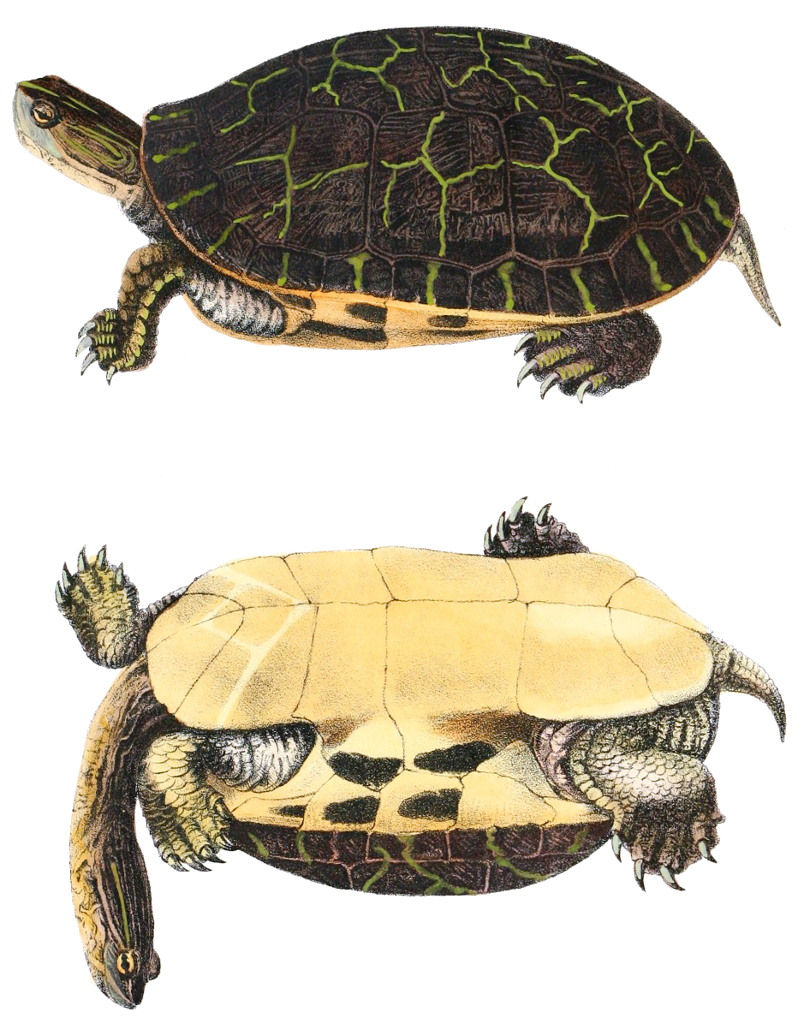
\includegraphics[scale=0.25]{testudines/emydidae/deirochelys/1}
\end{center}